\chapter{Graphical User Interface for PHAISTOS}

Setting up simulations in PHAISTOS requires expert knowledge about the program. 
Firstly, while all modules and settings have reasonable default settings, there are still many things that cannot be specified via default alone, and secondly, the complete list of settings in PHAISTOS is around 2500 options that must be set or taken as default values.

In order to make PHAISTOS more attractive to new users, I wrote a GUI can set up most simulations for most of the simulations covered by this thesis.
The GUI for PHAISTOS is aptly named Guistos and is written in Python 2.x using TkInter.

Using the GUI the user is only presented with the three most basic choices for setting up the simulation.
These are (1) choice of energy terms, (2) type of Monte Carlo simulation and finally (3) a selection of Monte Carlo moves.
A screenshot of Guistos can be seen in Fig.~\ref{fig:guistos}.
Setting up these via Guistos is discussed below.

\begin{figure}
    \centering
    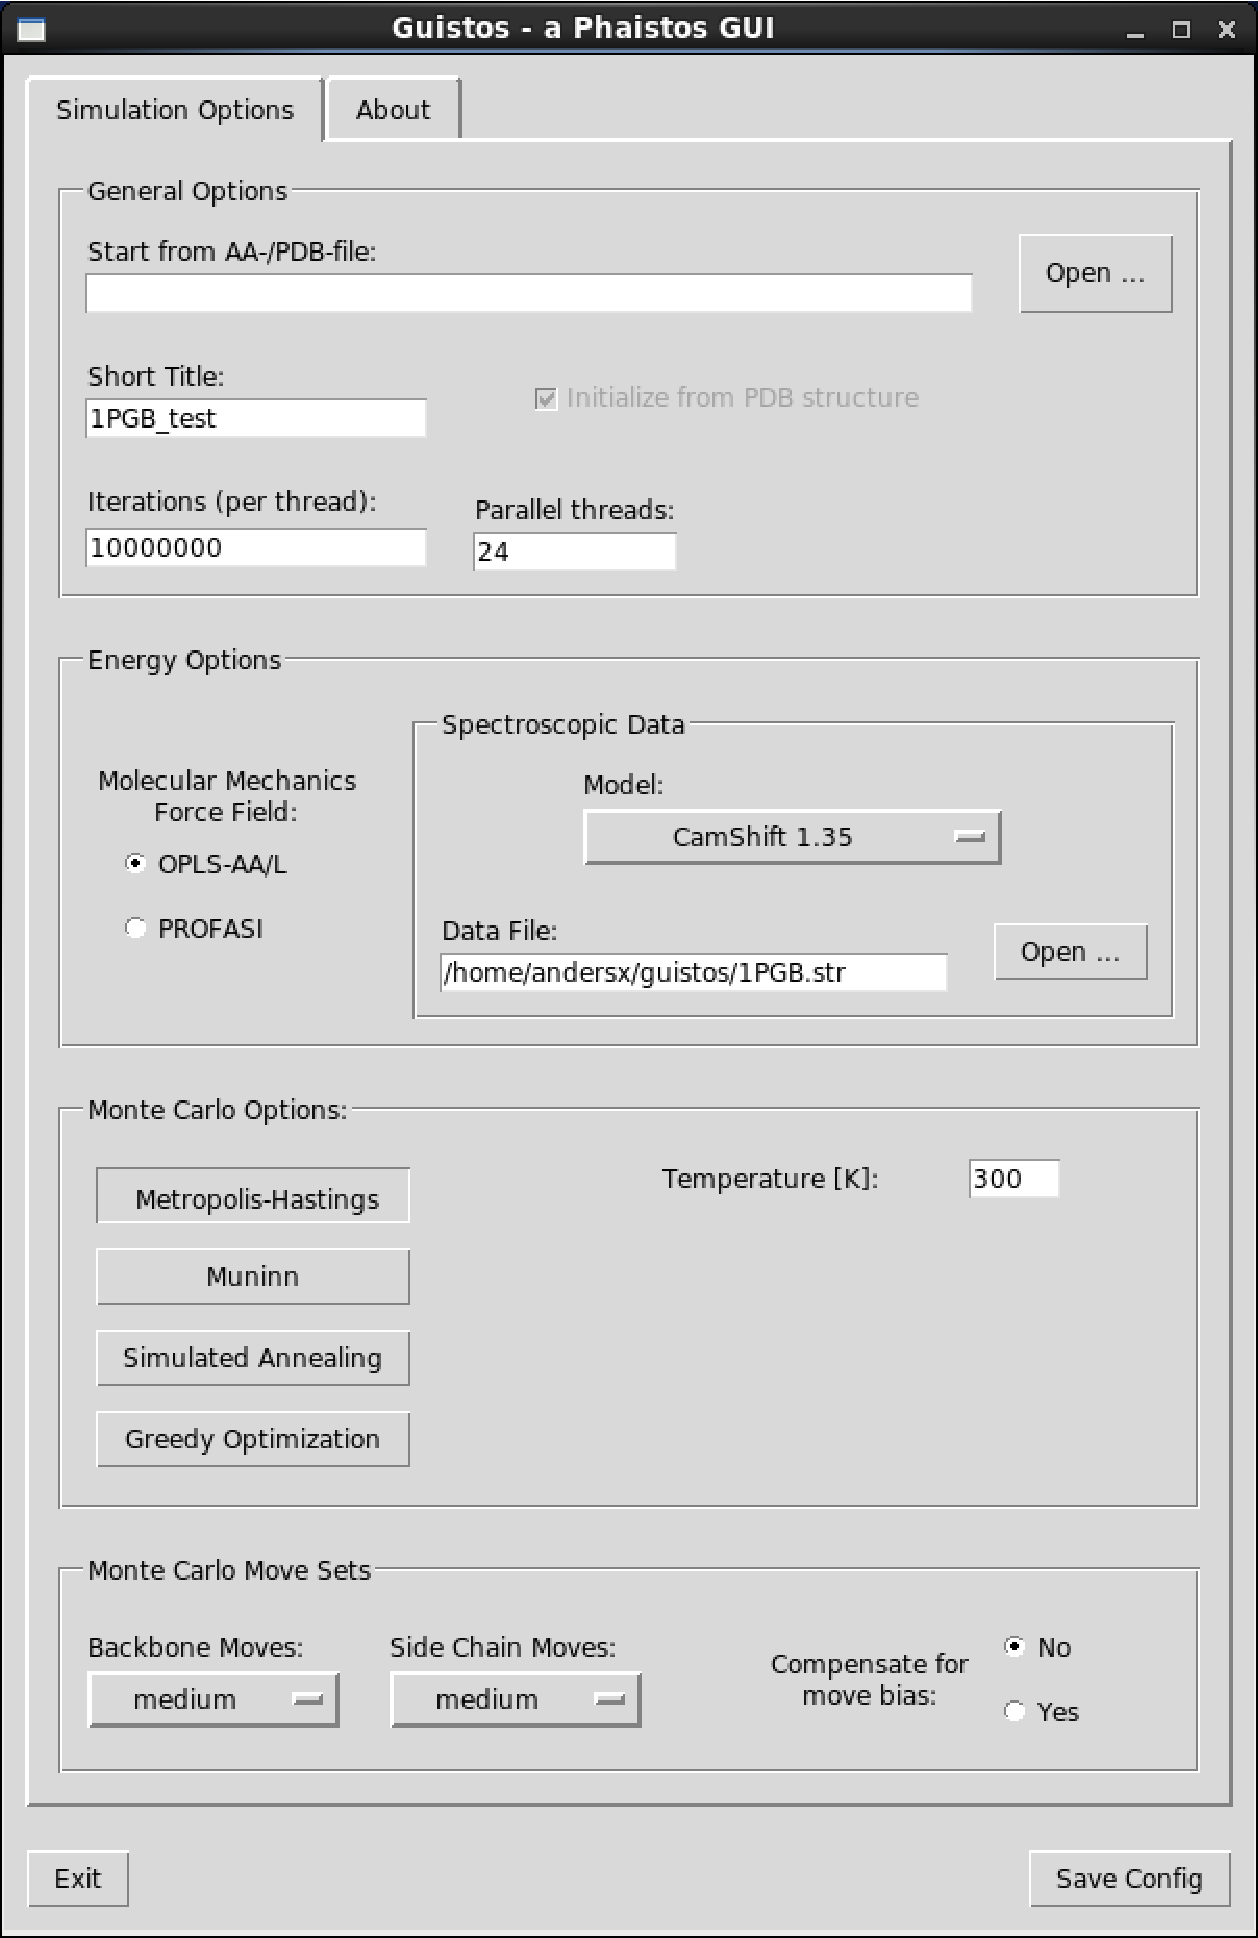
\includegraphics[width=0.70\textwidth]{figures/guistos.pdf}
    \caption{Screenshot of Guistos}
    \label{fig:guistos}
\end{figure}

\subsubsection{Energy Options}

Firstly, the Energy Options section allows the user to select the molecular mechanics force field.
Currently two force fields are supported in PHAISTOS, which are the OPLS-AA/L force field with a GB/SA solvent model, and the PROFASI coarse grained force field.
Use of the PROFASI force field requires the Monte Carlo moves to restraint the bond angle and lengths in the protein to Engh-Huber standard values.
This is automatically done if the PROFASI force field is selected. 
Conversely, the OPLS-AA/L force field includes energy terms for bond angles and lengths and these are degrees of freedom in the simulation if the OPLS-AA/L force field is selected.

Additionally, the Energy Options section allows the user to add restrains from one type spectroscopic data.
Currently energy terms based on CamShift 1.35 and ProCS are supported.
These options requires a NMR-STAR formatted file containing experimental chemical shifts.


\subsubsection{Monte Carlo Options}

This section allows the user to select the four types of Monte Carlo simulation offered by PHAISTOS and the only the most basic options to set up that particular simulation:
Metropolis-Hastings offers the choice of a constant temperature (in Kelvin).
Muninn and Simulated Annealing offer the choice of a temperature range (in Kelvin), and additionally Muninn offers the choice between multicanonical or $1/k$ sampling.
Greedy Optimization does not offer any customizable option. 

\subsubsection{Monte Carlo Move Sets}

Selecting a good mix of the different Monte Carlo moves offered by PHAISTOS can significantly speed up convergence of a simulation, compared to using an inferior move set.
Choosing a good set of moves is in the opinion of this author currently somewhere in between black art and sheer luck, and requires a good deal of experience with simulations in PHAISTOS.

To make it easier for new users, three move sets have been predefined using the experience of this author.
These are named "small", "medium" and "large".
The "small" move set is intended for uses such as refinement or sampling around a compact native state, 
while the "medium" move set is intended for folding simulations that start from extended, but are expected to also sample a native state, 
and finally the "large" move set is intended for sampling conformational space quickly, but will have problems with sampling compact structures.
All move sets sample from TorusDBN (backbone angles) and BASILISK (side chain angles), and an option to remove this bias is also present.

\subsubsection{Using Guistos}

Guistos is freely released under the open source two-clause BSD-license, and can be downloaded from \url{https://github.com/andersx/guistos}. After specifying all relevant settings in the Guistos window, a configuration-file is saved by pressing the "Save Config" button.
A simulation in PHAISTOS can the be executed via the following command:
\begin{lstlisting}
./phaistos --config-file my_simulation.config
\end{lstlisting}







